\chapter{Werken met React Native} \label{chapter:workrn}
Facebook en de community werken hard om het React Native framework grondig uit te bouwen en alle platform specifieke componenten en \hyperref[api]{API's} te integreren. In dit hoofdstuk worden een aantal van deze componenten en \hyperref[api]{API's} besproken die resulteren in een applicatie als voorbeeld.  
\section{Werkomgeving}
\subsection{MAC OSX}
Applicaties ontwikkelen voor iOS met React Native kan momenteel enkel gebeuren in een MAC OSX omgeving, omdat native iOS applicaties enkel ontwikkeld kunnen worden in \emph{XCode}, de ontwikkelomgeving van MAC OSX. Om deze omgeving compatibel te maken met React Native zijn een aantal stappen vereist. 

Eerst en vooral raadt Facebook aan om \emph{Homebrew} te installeren. \emph{Homebrew} installeert pakketten en ontwikkelaars tools die Apple is vergeten. Deze pakketbeheerder installeren kan op eenvoudige manier in de \emph{terminal} door het commando : 
\begin{itemize}
	\item [] \emph{ruby -e ``\$(curl -fsSL https://raw.githubusercontent.com/Homebrew /install/master/install)''}
\end{itemize}

Wanneer \emph{Homebrew} is geïnstalleerd, kan het commando \emph{brew} gebruikt worden. Voor React Native is het ook verplicht om \emph{Node.js v4.0} of recenter te gaan installeren. Hiervoor is de \emph{Node Version Manager of nvm} nodig. Deze wordt standaard geïnstalleerd wanneer XCode wordt geïnstalleerd. Om \emph{Node.js} te installeren gebruik het commando : 
\begin{itemize}
\item [] \emph{nvm install node \&\& nvm alias default node}
\end{itemize}
Deze zal de laatste nieuwe versie van \emph{Node.js} installeren. \emph{Node.js} is nodig om de applicatie te runnen op de simulator en zorgt er ook voor dat de Javascript ontwikkelaar tools beschikbaar worden. 
Om te voorkomen dat er fouten zijn tijdens het ontwikkelingsproces wanneer \emph{Node.js} server draait en de code wordt aangepast, werd \emph{Watchman} door Facebook ontwikkeld. \emph{Watchman} gaat het project observeren en de nodige scripts oproepen wanneer de code wordt aangepast tijdens het ontwikkelingsproces. Installeer \emph{Watchman} door gebruik te maken van het volgende commando : 
\begin{itemize}
	\item [] \emph{brew install watchman}
\end{itemize}  
Optioneel raden de ingenieurs van Facebook aan om \emph{Flow} te gaan gebruiken. \emph{Flow} gaat type errors detecteren in Javascript programma's en werd door Facebook ontwikkeld. Het kan via het \emph{Homebrew} commando worden geïnstalleerd : 
\begin{itemize}
	\item [] \emph{brew install flow}
\end{itemize}
Wanneer deze stappen zijn uitgevoerd, is de iOS omgeving klaar om React Native te installeren. Voor Android is de installatie van Android \hyperref[sdk]{SDK} uiteraard verreist. Wanneer ook de Android omgeving werd geconfigureerd volgens de stappen die Google voorziet in de documentatie, kan er ook een \hyperref[emulator]{emulator} van een Android compatibel toestel worden aangemaakt dat nodig is om de applicaties te laten draaien.

Het installeren van React Native gebeurt door het volgende commando : 
\begin{itemize}
	\item [] \emph{npm install -g react-native-cli}
\end{itemize}

\subsection{Windows en Linux}
Ontwikkelen van applicaties met React Native kan in beperkte mate ook op Windows en Linux maar enkel voor Android-applicaties. Facebook besteedt hiervoor het beheer en de opvolging uit aan de community van React Native. De reden hiervoor is dat de ingenieurs bij Facebook gebruik maken van MAC OSX en dus krijgt de ondersteuning voor OSX prioriteit. Men gelooft bij Facebook dat de beste Linux en Windows ondersteuning dan ook enkel kan komen van mensen die dagelijks met deze \hyperref[os]{OS} werken. \citep{facebook:ReactNative}
Ook in deze scriptie wordt gebruik gemaakt van MAC OSX en zal verder niet meer verwezen worden naar het gebruik voor Windows of Linux.
\subsection{Start React Native}
Om een nieuw project te starten in React Native wordt volgende commando gebruikt : 
\begin{itemize}
	\item [] \emph{react-native init HelloWorld}
\end{itemize}
Dit zal een map plaatsen in het filesysteem met de naam \emph{HelloWorld}. Deze map bevat reeds 2485 directories en 10660 files. Op \prettyref{fig:map} wordt de inhoud van de map weergegeven. De mappen \emph{android} en \emph{ios} bevatten \hyperref[boilerplate]{boilerplate code} relevant aan het platform, deze zijn ook de respectievelijke startpunten van de applicaties. In de \emph{node\_modules} map worden de \emph{node} afhankelijkheden die werden geïstalleerd via \emph{npm} opgeslagen. De documenten \emph{index.ios.js} en \emph{index.android.js} bevatten de React code die de views van de applicaties beschrijven, \prettyref{code:index}. Wanneer in XCode het project uit de map \emph{ios} wordt geopend en de iPhone emulator opgestart, start de applicatie en zal de view die in de \emph{render} functie van de \emph{HelloWorld} component weergegeven worden, \prettyref{fig:simulator}. Hetzelfde kan met een Android emulator ook gebeuren door in de \emph{terminal} naar de \emph{android} map te gaan en daar het commando te gebruiken om de android applicatie te starten : 
\begin{itemize}
	\item [] \emph{react-native run-android}
\end{itemize}

		\reactcode{code/index.android.js}{HelloWorld gegenereerde code}{code:index}

\begin{figure}%
\centering
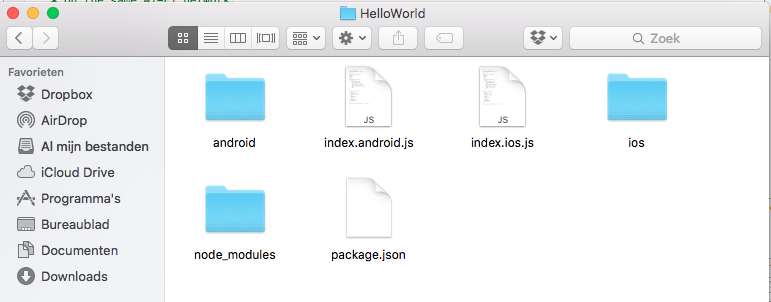
\includegraphics[width=.8\columnwidth]{img/HelloWorld.png}%
\caption{Schermafbeelding map HelloWorld project}%
\label{fig:map}%
\end{figure}

\begin{figure}%
\centering
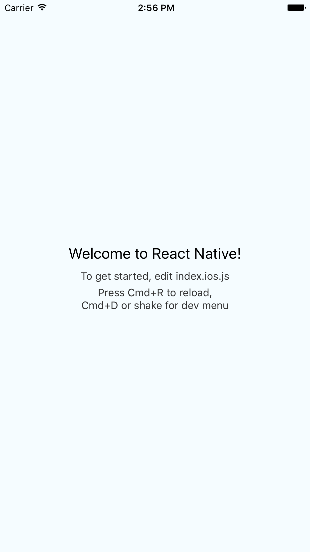
\includegraphics[width=0.5\columnwidth]{img/simulator.png}%
\caption{HelloWorld op iOS simulator}%
\label{fig:simulator}%
\end{figure}

De applicaties kunnen nu aangepast worden in de \emph{index.xxx.js} files. Door de emulators te laten herladen worden de wijzigingen zichtbaar. \citep{getstarted:ReactNative}


\section{Componenten}
\hyperref[ui]{UI} Componenten vormen de basis van een applicatie in React Native en verwijzen naar platform specifieke elementen. Er wordt dan ook een onderscheid gemaakt tussen \emph{cross-platform componenten} en \emph{platform specifieke componenten} met elk hun eigen manier van werken. Het is ook gebruikelijk om componenten in eigen \emph{.js} documenten te plaatsen om bepaalde principes van \hyperref[oo]{OO} te kunnen gebruiken. Componenten kunnen herbruikt worden en het geheel blijft overzichtelijk, \prettyref{fig:mappen}. Om een component te importeren uit een ander Javascript document moet \emph{require} worden aangeroepen gevolgd door de locatie van het document, \prettyref{code:import}. 

		\reactcode{code/import.js}{Importeren van componenten}{code:import}


\begin{figure}%
\centering
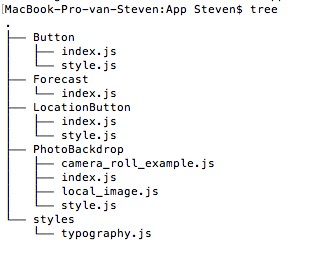
\includegraphics[width=0.5\columnwidth]{img/mappen.png}%
\caption{Mappen structuur voor applicatie}%
\label{fig:mappen}%
\end{figure}

\subsection{Cross-platform componenten}
  
	\emph{Cross-platform componenten} zijn componenten die voor beide platform gelijkwaardig worden behandeld en worden als basis componenten aanzien. 
	\subsubsection{Text}
	Een voorbeeld hiervan is het \emph{<Text>} component. Zoals de naam doet vermoeden is dit een wrapper component die een tekst zal bevatten om af te printen op het scherm. Werken met tekst in React Native is eenvoudig maar verschillend in hoe het werkt in webontwikkeling. Het is mogelijk om daar tekst te plaatsen zonder een specifieke wrapper maar in native ontwikkeling is dit een verplichte tag om tekst te gaan gebruiken. In \prettyref{code:text} wordt een voorbeeld weergegeven hoe in React Native een \emph{text} tag gebruikt wordt. In React Native bestaan er geen componenten zoals \emph{<h1> of <h2>}, deze kunnen gemakkelijk nagebootst worden door een stijl klasse mee te geven en de \emph{fontsize} aan te passen.\citep{api:ReactNative} 
			\reactcode{code/rntext.js}{Voorbeeld gebruik van Text}{code:text}
		\subsubsection{Image}	
Het \emph{text} component is het meest eenvoudige component in React Native gevolgd door het \emph{image} component. Met \emph{image} kan een afbeelding weergegeven worden op het scherm, dit kan op een aantal verschillende manieren.
In \prettyref{code:require} wordt getoond hoe een afbeelding uit het file systeem van de Android of iOS \emph{package} gebruikt kan worden. Deze moeten volgens de richtlijnen van respectievelijk Android en iOS ontwikkeling worden toegevoegd aan de correcte folders. In hetzelfde voorbeeld wordt ook getoond hoe een afbeelding kan gebruikt worden als achtergrond met bijvoorbeeld een tekst op de voorgrond. Dit wordt mogelijk gemaakt doordat React Native werkt met componenten, en deze als een container kan gebruikt worden om andere componenten in te gaan wrappen.     
			\reactcode{code/image.require.js}{Voorbeeld gebruik van Image met require}{code:require}
			\reactcode{code/image.uri.js}{Voorbeeld gebruik van Image met Uri}{code:uri}

Een andere manier om een afbeelding te gaan gebruiken, is om het te downloaden van het internet. Hiervoor wordt een uri meegegeven zoals in \prettyref{code:uri}. Let wel, wanneer een afbeelding wordt gedownload, moet er verplicht een dimensie meegegeven worden, anders wordt de afbeelding niet zichtbaar.\citep{api:ReactNative}

\subsubsection{ListView}
Naast \emph{text} en \emph{image} wordt in native ontwikkeling heel veel gebruik gemaakt van lijsten die weergegeven worden dankzij een \emph{ListView} component in React Native. In \prettyref{code:basislv} wordt een basis implementatie van een \emph{ListView} getoond. Er zijn een aantal verplichtingen bij het gebruik van \emph{ListView}, zo wordt in het voorbeeld in \emph{getInitialState} eerst een \emph{ListView.DataSource} object aangemaakt die een functie \emph{rowHasChanged} meekrijgt. Deze zal als een \hyperref[observer]{Observer} fungeren op de lijst en detecteren wanneer een lijstitem moet aangepast worden. Daarnaast wordt een \emph{state} object, \emph{dataSource} geïnitialiseerd met het \emph{ListView.DataSource} object met een array in de \emph{cloneWithRows} functie. In de \emph{render} functie wordt de \emph{ListView} vervolgens opgevuld met een \emph{dataSource} die uit de state gehaald wordt en wordt in \emph{renderRow} aangegeven welk item er rij per rij wordt weergegeven.\citep{api:ReactNative}

		\reactcode{code/listview.js}{Voorbeeld gebruik van basis ListView }{code:basislv}

\subsubsection{Touch}
Een van de basis componenten die men kan gebruiken om een \emph{TouchEvent} op te vangen, is het \emph{TouchableHighlight} component. Deze kan rond een \emph{View} of andere component worden geplaatst en zal één of meer van volgende methoden moeten bevatten : \emph{onPressIn, onPressOut, onLongPress, onPress, ...} . Het gebruik ervan is simpel en wordt getoond in \prettyref{code:thl}. In dit voorbeeld zal de tekst die verschijnt op de knop wijzigen wanneer een bepaald drukbeweging wordt uitgevoerd.\citep{api:ReactNative}
	
		\reactcode{code/thl.js}{Voorbeeld gebruik van basis TouchableHighLight}{code:thl}
		
		\subsection{Platform specifieke componenten}
Platform specifieke componenten kunnen herkend worden aan de prefix, meestal wordt het platform aangegeven als deel van de naam van het component. Platformspecifieke componenten zijn heel vaak nodig omdat niet alle componenten eenzelfde tegenhanger hebben op elk platform. Het kan ook zijn dat een bepaald component wel cross-platform is maar een bepaalde \emph{property} niet. Zo kan je in iOS op component \emph{TextInput}, \emph{property : maxLength} gebruiken en op Android niet. Dit wordt in de \hyperref[api]{API} van React Native weergegeven door een label. \citep{api:ReactNative}.

Wanneer platformspecifieke componenten worden aangemaakt, moet er nauw opgelet worden dat deze in de correcte file worden geïmporteerd, zoniet zal de applicatie stoppen met werken. Componenten \emph{<SwitchAndroid> en <SwitchIOS>} zijn 2 componenten die in elk platform specifiek moeten worden aangemaakt, op \prettyref{fig:switch} wordt de file structuur afgebeeld. Hier wordt een onderscheid gemaakt tussen \emph{switch.android.js}, \prettyref{code:sAndroid} en \emph{switch.ios.js}, \prettyref{code:siOS} welke respectievelijk een \emph{switch} component aanmaken voor Android en iOS. In \emph{crossPlatform.js}, \prettyref{code:cross} wordt de \emph{switch} geïmporteerd, merk op dat er geen \emph{.android of .ios} na \emph{switch} wordt geplaatst. De native compiler van React Native gaat dit voor de ontwikkelaar bepalen welke \emph{switch} wordt ingeladen afhankelijk van het platform.

		\begin{figure}%
		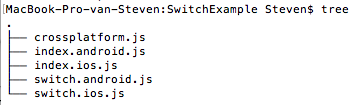
\includegraphics[width=\columnwidth]{img/switch.png}%
		\caption{Map structuur van SwitchExample}%
		\label{fig:switch}%
		\end{figure}
				\reactcode{code/switch.android.js}{Switch voorbeeld specifiek voor Android}{code:sAndroid}
				\reactcode{code/switch.ios.js}{Switch voorbeeld specifiek voor iOS}{code:siOS}
				\reactcode{code/crossplatform.js}{Crossplatform import Switch}{code:cross}
\emph{Switch} is een voorbeeld van een component die zowel voor Android als voor iOS kan gebruikt worden op dezelfde manier en toch verschillend geïmplementeerd worden door de \emph{native compiler} van React Native. Sommige componenten zijn uiteraard enkel op een specifiek platform te verkrijgen, zoals de \emph{<TabBarIOS>} die een navigatie item onderaan de applicatie plaatst, \prettyref{fig:tabbar}. Voor Android kan de ontwikkelaar in dit geval kiezen voor een \emph{<ToolBarAndroid>} component of voor een \emph{<DrawerLayoutAndroid>} component. Deze werkwijze zorgt ervoor dat sommige code niet herbruikbaar is en dat de ontwikkelaar goed moet opletten dat de code van de platform-specifieke componenten gescheiden blijft.  
																
																\begin{figure}%
																\centering
																
\includegraphics[width=0.5\columnwidth]{img/tabbarios}%
																\caption{TabBarIOS voorbeeld}%
																\label{fig:tabbar}%
																\end{figure}
																
	\subsubsection{Native UI componenten}
Er zijn momenteel heel wat native UI componenten aanwezig in het React Native platform en ook als \emph{third-party libraries} aangeboden door leden uit de community. Maar soms kunnen ontwikkelaars eigen UI componenten ontwikkelen die applicatie- of bedrijfs specifiek zijn, dan biedt React Native nog een ander alternatief aan, namelijk het \emph{custom} component zelf aanmaken in Objective C of Java en exporteren naar Javascript. Dit kan door een standaard Objective C of Java object aan te maken die een \emph{View} voorstelt. De Java klasse zal moeten overerven van \emph{SimpleViewManager} en de Objective C klasse van \emph{RTCViewManager}, om de export mogelijk te maken. Methoden en properties worden geannoteerd volgens de annotaties voorzien in de superklasse, zodat ze kunnen gebruikt worden in Javascript. Wanneer de ontwikkelaar zijn componenten wenst te gebruiken, hoeft hij die enkel nog te importeren. De brug van React Native voorziet hiervoor een aantal klassen die dit voor de ontwikkelaar gaat opvangen, aan de hand van de annotaties die werden geplaatst.

Wanneer is het een goed idee om native Objective-C of Java code te gaan gebruiken? 
\begin{itemize}
	\item Wanneer er reeds een bestaande native applicatie is, kan het nuttig zijn bepaalde modules te exporteren om zo dubbel werk te voorkomen.
	\item Wanneer de applicatie gespecialiseerde taken met een hoog CPU gebruik moet gaan uitvoeren, wordt het aangeraden om deze in de Objective-C of Java te laten uitvoeren en het resultaat ervan naar de Javascript view doorgegeven.
	\item En wanneer er tenslotte nog geen ondersteuning is voor een platform specifiek component of API. React Native is momenteel in actieve ontwikkeling en ook Android en iOS zullen blijven innoveren.
\end{itemize}

	\section{API}
Het grote voordeel van native ontwikkeling is het gebruik van de hardware componenten van het toestel waarop de applicatie draait, hiervoor zal de ontwikkelaar gebruik willen maken van de verschillende \hyperref[api]{API's} die voor het platform worden aangeboden. Die \hyperref[api]{API's} worden toegankelijk voor React Native door modules (reeds aanwezig in de \emph{node\_modules} map) die de ontwikkelaar voorzien van Javascript interfaces die de API's asynchroon gaan aanspreken. Uiteraard zijn er ook API modules die cross-platform zijn en die platform specifiek zijn. Door de complexiteit van sommige API's heeft React Native niet altijd alle functionaliteiten in het platform geïntegreerd, sommige onderdelen worden door de community aangereikt en in sommige gevallen zal de ontwikkelaar de modules zelf moeten ontwikkelen in Objective-C of Java. Het spreekt dan ook voor zich dat er zowel cross-platform API modules bestaan als platform specifieke API modules.
 
\subsection{Cross-platform API modules}
De lijn tussen cross-platform en platformspecifieke API modules is erg dun. Een module die nu momenteel slechts op één platform beschikbaar is, kan binnen enkele weken (of zelfs dagen) cross-platform gemaakt worden aangezien Facebook en de community nog steeds actief bezig zijn om het platform te verbeteren. 
\subsubsection{AsyncStorage}
Een eerste en belangrijke module is de \emph{AsyncStorage}, een simpel persistentie systeem die over de globale applicatie gebruikt kan worden. \emph{AsyncStorage} kan vergeleken worden met \emph{LocalStorage} die gebruikt wordt in webontwikkeling. Aangezien de werkwijze van \emph{AsyncStorage} gelijkaardig is met die van \emph{LocalStorage} kan een webontwikkelaar hieraan snel gewoon raken. De data wordt via een Javascript systeem opgeslagen in het intern geheugen als \hyperref[json]{json-object}. In \prettyref{code:save} en \prettyref{code:retrive} wordt getoond hoe data wordt opgeslagen en terug opgevraagd aan de hand van de \emph{key}. Dit gebeurt volledig asynchroon waardoor de applicatie niet nodeloos belast wordt. 

\reactcode{code/savedata.js}{AsyncStorage: opslaan van data}{code:save}
\reactcode{code/retrivedata.js}{AsyncStorage: opvragen van data}{code:retrive}
	
	\subsubsection{PanGesture}
Naast data opslaan, kan het voor een ontwikkelaar interessant zijn om gebruik te maken van de aanrakingsmogelijkheden van smartphones en tablets. Hiervoor heeft React Native een \emph{PanGesture} module ontwikkeld. Deze gaat de aanrakingen van de gebruiker kunnen behandelen en laten resulteren in gepaste wijzigingen op het scherm. Omdat aanrakingen op mobiel anders zijn dan die op het web voorziet React Native een interface voor \emph{PanGesture} die de methoden nodig voor de implementatie onmiddellijk meegeeft, deze kunnen door de ontwikkelaar overschreven worden om het gewenste resultaat te bekomen. In \prettyref{code:pan} wordt de \emph{\_handlePanResponderMove} overschreven, in dit voorbeeld zal een cirkel, wanneer die versleept wordt door de gebruiker, van plaats veranderen. Dankzij het \emph{gestureState} object die de locatie van de aanraking op het scherm bijhoudt, kan de locatie van de cirkel worden aangepast in de update functie.

 \reactcode{code/pangesture.js}{PanGesture voorbeeld}{code:pan}

\subsection{Platform specifieke API modules}
Uiteraard zijn de meeste API modules platform specifiek, dit komt doordat Apple en Google andere functionaliteiten in hun platform integreren. Zo heeft Android bijvoorbeeld een \emph{Toast} API die de gebruiker onderaan het scherm een bericht kan geven. Hiervoor kan bij React Native de \emph{ToastAndroid} module gebruikt worden, deze kan op eenvoudige wijze worden aangesproken, \prettyref{code:toast}. Deze code zal bijvoorbeeld na een \emph{onPress()} functie van een knop een toast op het scherm afbeelden, \prettyref{fig:toast}. Hetzelfde kan voor iOS door middel van bijvoorbeeld een \emph{AlertIOS} te implementeren. Bij \prettyref{code:alert} zal de \emph{onPress} functie een standaard iOS \emph{alert} venster op het scherm afbeelden, \prettyref{fig:alert}. In dit geval gebeurt dat met een \emph{default button} die het venster opnieuw terug afsluit. Wanneer er aan de \emph{alert} een array met een reeks van objecten, die een title en een \emph{onPress} functie bevatten, wordt meegegeven, zal op basis hiervan een reeks knoppen aan het \emph{alert} venster worden meegegeven.   

 \reactcode{code/toast.js}{ToastAndroid voorbeeld}{code:toast}

\begin{figure}%
\centering
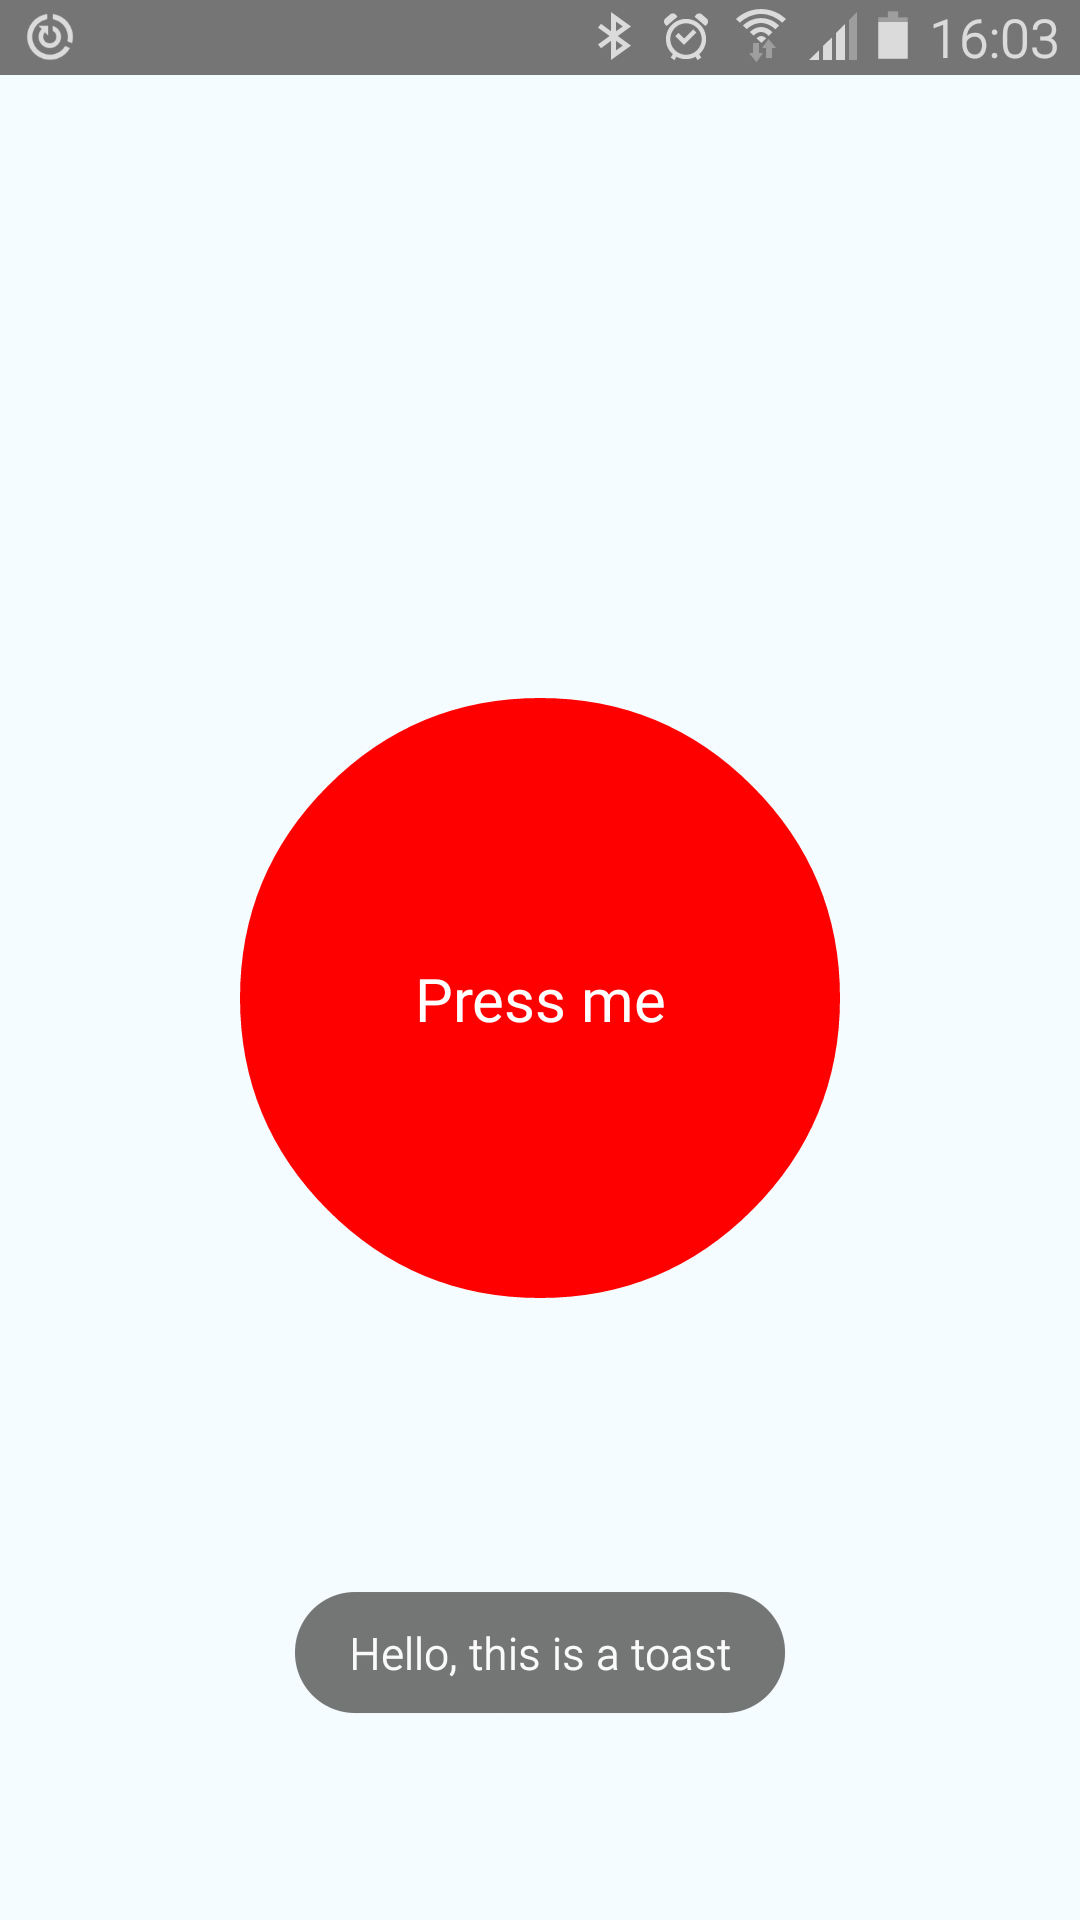
\includegraphics[width=0.5\columnwidth]{img/toast.png}%
\caption{ToastAndroid schermafbeelding}%
\label{fig:toast}%
\end{figure}

 \reactcode{code/alertios.js}{AlertIOS voorbeeld}{code:alert}

\begin{figure}%
\centering
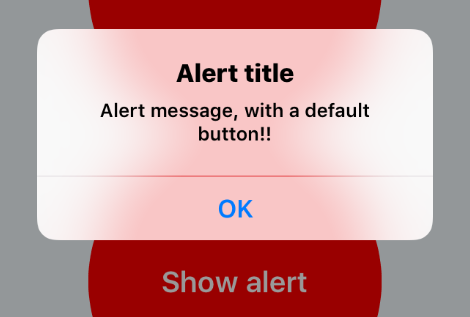
\includegraphics[width=0.5\columnwidth]{img/alert.png}%
\caption{AlertIOS schermafbeelding}%
\label{fig:alert}%
\end{figure}

\section{Debuggen en testen}
React Native werd ontwikkeld om webontwikkelaars de kans te geven om native applicaties te schrijven, Facebook heeft er dan ook voor gezorgd dat het debuggen van de applicatie lijkt op het debuggen van een webapplicatie. Hiervoor zijn een aantal mogelijkheden, de combinatie van meerdere debug manieren is dan ook aangeraden net zoals in webontwikkeling. 

\subsection{Ontwikkelaars opties}
Wanneer een applicatie wordt afgespeeld op een simulator of op een echt toestel dan kan er een menu worden aangesproken die een aantal opties geeft aan de ontwikkelaar, \prettyref{fig:devtools}. In dit menu kan de ontwikkelaar elementen inspecteren, net zoals dat kan in de chrome of safari ontwikkelingstools, de applicatie opnieuw laten inladen of de chrome Javascript debug tool gebruiken om \hyperref[breakpoint]{breakpoints} te detecteren. Wanneer de applicatie om een bepaalde reden vastloopt is er een \emph{Red Screen of Death} te zien voor de ontwikkelaar, dit scherm geeft de reden van het vastlopen van de applicatie op een betekenis volle manier terug zoals op \prettyref{fig:redscreen}.   
	
	\begin{figure}%
	\centering
	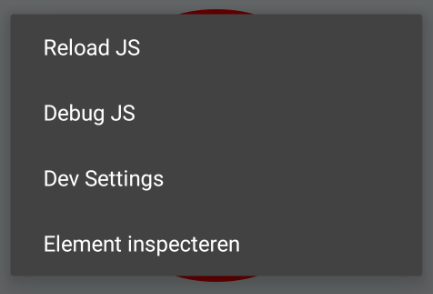
\includegraphics[width=.5\columnwidth]{img/devtools.png}%
	\caption{In-app ontwikkelaars opties}%
	\label{fig:devtools}%
	\end{figure}
	
	\begin{figure}%
	\centering
	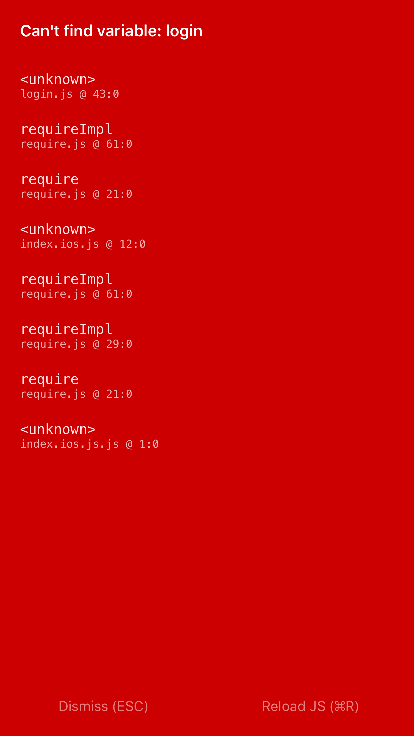
\includegraphics[width=0.5\columnwidth]{img/redscreen.png}%
	\caption{The Red Screen of Death}%
	\label{fig:redscreen}%
	\end{figure}
	
Naast de mogelijkheid om te debuggen in de applicatie zelf, kunnen de chrome en safari development tools ook gebruikt worden om de applicatie te debuggen. Aangezien de applicatie draait op een \emph{node.js} server kan de ontwikkelaar via \emph{http://localhost:8081} de applicatie debuggen in de browser. Er is ook geen enkele aanpassing nodig om te werken met \emph{console.log} waarvan de output in de Javascript console wordt weergegeven. Maar ook in Xcode zal de output van \emph{console.log} zichtbaar zijn voor de iOS applicatie. Voor de Android applicatie kan de ontwikkelaar \emph{logcat} activeren door in de hoofdmap van het project volgend commando te activeren : 
\begin{itemize}
	\item [] \emph{adb logcat}
\end{itemize}
De logs zullen in de \emph{terminal} verschijnen. Deze laatste optie voor Android geeft een onoverzichtelijk geheel van logs terug omdat de logs van platform-specifieke zaken hier ook worden weergegeven. \citep{eisenman:react}

Het is ook mogelijk gemaakt om, net zoals bij webontwikkeling, \hyperref[css]{CSS} componenten te gaan wijzigen wanneer de applicatie loopt en dit rechtstreeks in de browser, hiervoor hoeft de ontwikkelaar enkel de React plugin te downloaden voor chrome of safari. Deze functie is voor React Native momenteel nog in opbouw waardoor sommige functionaliteiten hiervoor nog niet helemaal of volledig niet werken.

\subsection{Testen}    			
Debuggen van de applicatie wil zeggen dat de ontwikkelaar een fout in zijn code zal moeten zoeken en oplossen, het is in applicatie ontwikkeling dan ook aan te raden om te voorkomen dat bepaalde \emph{bugs} voorkomen. Dit kan door testen te schrijven. Veel van de React Native code die geschreven wordt, is niet altijd code die uitsluitend gebruikt wordt voor mobiele applicatie ontwikkeling. Veel van de business logic code kan geïsoleerd worden van de render code. Op deze manier kan men Javascript code testen door gebruik te maken van om het even welke Javascript development tool.

React Native raadt een aantal tools aan voor ontwikkelaars die door de ingenieurs van Facebook zelf gebruikt (of ontwikkeld) zijn tijdens het ontwerpen van React Native. 

\subsubsection{Flow}
\emph{Flow} is een Javascript library voor \emph{static-type checking}. \emph{Flow} gaat de ontwikkelaar helpen met het vinden van errors op gebied van type interferentie. Wanneer een variabele een string object meekrijgt en er later een bewerking op gebeurt zoals op een nummer type, zal \emph{Flow} de ontwikkelaar waarschuwen. Om een check te doen van een React Native project hoeft de ontwikkelaar in de \emph{command line} volgend commando in te geven : 
\begin{itemize}
	\item [] \emph{flow check}
\end{itemize}  
De check zal op gepaste wijze aangeven of er al dan niet errors gevonden werden.

\subsubsection{Jest}
React Native ondersteunt testen van React componenten door middel van \emph{Jest}, een unit testing framework gebouwd op \emph{Jasmine}. Het voorziet aggresieve automocking van afhankelijkheden, en werkt perfect samen met de ontwikkelaars tools van React Native. Om \emph{Jest} te gebruiken moet dit uiteraard eerst geïnstalleerd worden :
\begin{itemize}
	\item [] npm install jes-cli --save-dev
\end{itemize}
Daarna kan de \emph{package.json} aangepast worden door een test script toe te voegen, \prettyref{code:package}. Wanneer \emph{npm test} wordt uitgevoerd zal deze met behulp van \emph{Jest} de tests doorlopen. In de hoofdmap moet een map komen, genaamd \emph{tests}. \emph{Jest} zal recursief opzoek gaan naar test documenten in \emph{tests/} map. \prettyref{code:jest} geeft een voorbeeld van een simpele test case. 


 \reactcode{code/package.js}{Voeg test script toe aan package.json}{code:package}
 \reactcode{code/jest.js}{Voorbeeld van Jest test}{code:jest}
